% =====================================================================
% preview_routing_share_mix_a -- R/ggplot2 -> tikzDevice (Frame-A, ESWA target)
% Canonical-JSON-only. Regenerate: Rscript submissions/frame-a-eswa/figures-r/make_figures_frame_a.R
% Provenance (JSON path :: field = plotted value), one line per series:
% SOURCE: results/frame_a/cells/cell_llama-3.2-1b_real_MIX_A_both_s{0,1,2}.json :: mean routing.arm_counts.grace / mean total = 0.9720
% SOURCE: results/frame_a/cells/cell_llama-3.2-1b_real_MIX_A_both_s{0,1,2}.json :: mean routing.arm_counts.edit / mean total = 0.0280
% =====================================================================
% WARNING: QA-PREVIEW-NOT-FOR-SUBMISSION (generated 2026-07-23 08:37:26 EDT)
% This file is NOT camera-ready. The MIX_A preview under figures-qa/
% !TEX encoding = UTF-8 Unicode
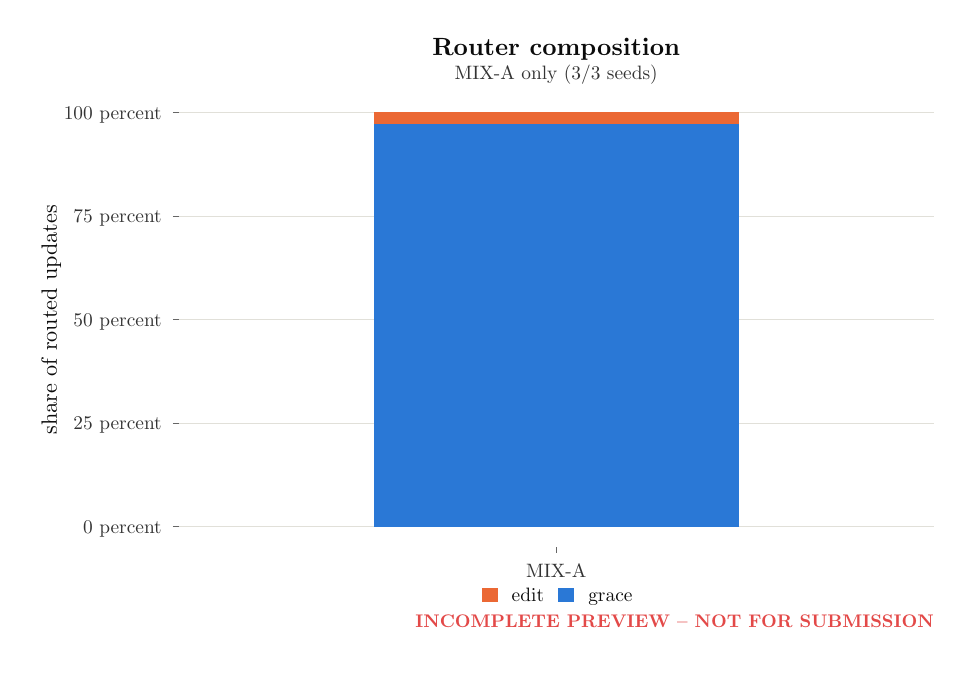
\begin{tikzpicture}[x=1pt,y=1pt]
\definecolor{fillColor}{RGB}{255,255,255}
\path[use as bounding box,fill=fillColor,fill opacity=0.00] (0,0) rectangle (332.44,224.04);
\begin{scope}
\path[clip] (  0.00,  0.00) rectangle (332.44,224.04);
\definecolor{fillColor}{RGB}{255,255,255}

\path[fill=fillColor] ( -0.00,  0.00) rectangle (332.44,224.04);
\end{scope}
\begin{scope}
\path[clip] ( 54.51, 36.25) rectangle (327.44,200.89);
\definecolor{drawColor}{RGB}{225,224,217}

\path[draw=drawColor,line width= 0.3pt,line join=round] ( 54.51, 43.74) --
	(327.44, 43.74);

\path[draw=drawColor,line width= 0.3pt,line join=round] ( 54.51, 81.15) --
	(327.44, 81.15);

\path[draw=drawColor,line width= 0.3pt,line join=round] ( 54.51,118.57) --
	(327.44,118.57);

\path[draw=drawColor,line width= 0.3pt,line join=round] ( 54.51,155.99) --
	(327.44,155.99);

\path[draw=drawColor,line width= 0.3pt,line join=round] ( 54.51,193.41) --
	(327.44,193.41);
\definecolor{fillColor}{RGB}{42,120,214}

\path[fill=fillColor] (125.02, 43.74) rectangle (256.94,189.22);
\definecolor{fillColor}{RGB}{235,104,52}

\path[fill=fillColor] (125.02,189.22) rectangle (256.94,193.41);
\end{scope}
\begin{scope}
\path[clip] (  0.00,  0.00) rectangle (332.44,224.04);
\definecolor{drawColor}{gray}{0.20}

\node[text=drawColor,anchor=base east,inner sep=0pt, outer sep=0pt, scale=  0.70] at ( 48.46, 41.32) {0 percent};

\node[text=drawColor,anchor=base east,inner sep=0pt, outer sep=0pt, scale=  0.70] at ( 48.46, 78.74) {25 percent};

\node[text=drawColor,anchor=base east,inner sep=0pt, outer sep=0pt, scale=  0.70] at ( 48.46,116.16) {50 percent};

\node[text=drawColor,anchor=base east,inner sep=0pt, outer sep=0pt, scale=  0.70] at ( 48.46,153.58) {75 percent};

\node[text=drawColor,anchor=base east,inner sep=0pt, outer sep=0pt, scale=  0.70] at ( 48.46,191.00) {100 percent};
\end{scope}
\begin{scope}
\path[clip] (  0.00,  0.00) rectangle (332.44,224.04);
\definecolor{drawColor}{gray}{0.40}

\path[draw=drawColor,line width= 0.3pt,line join=round] ( 52.51, 43.74) --
	( 54.51, 43.74);

\path[draw=drawColor,line width= 0.3pt,line join=round] ( 52.51, 81.15) --
	( 54.51, 81.15);

\path[draw=drawColor,line width= 0.3pt,line join=round] ( 52.51,118.57) --
	( 54.51,118.57);

\path[draw=drawColor,line width= 0.3pt,line join=round] ( 52.51,155.99) --
	( 54.51,155.99);

\path[draw=drawColor,line width= 0.3pt,line join=round] ( 52.51,193.41) --
	( 54.51,193.41);
\end{scope}
\begin{scope}
\path[clip] (  0.00,  0.00) rectangle (332.44,224.04);
\definecolor{drawColor}{gray}{0.40}

\path[draw=drawColor,line width= 0.3pt,line join=round] (190.98, 34.25) --
	(190.98, 36.25);
\end{scope}
\begin{scope}
\path[clip] (  0.00,  0.00) rectangle (332.44,224.04);
\definecolor{drawColor}{gray}{0.20}

\node[text=drawColor,anchor=base,inner sep=0pt, outer sep=0pt, scale=  0.70] at (190.98, 25.38) {MIX-A};
\end{scope}
\begin{scope}
\path[clip] (  0.00,  0.00) rectangle (332.44,224.04);
\definecolor{drawColor}{RGB}{11,11,11}

\node[text=drawColor,rotate= 90.00,anchor=base,inner sep=0pt, outer sep=0pt, scale=  0.80] at ( 10.51,118.57) {share of routed updates};
\end{scope}
\begin{scope}
\path[clip] (  0.00,  0.00) rectangle (332.44,224.04);
\definecolor{fillColor}{RGB}{235,104,52}

\path[fill=fillColor] (164.00, 16.42) rectangle (169.83, 21.44);
\end{scope}
\begin{scope}
\path[clip] (  0.00,  0.00) rectangle (332.44,224.04);
\definecolor{fillColor}{RGB}{42,120,214}

\path[fill=fillColor] (191.66, 16.42) rectangle (197.50, 21.44);
\end{scope}
\begin{scope}
\path[clip] (  0.00,  0.00) rectangle (332.44,224.04);
\definecolor{drawColor}{RGB}{11,11,11}

\node[text=drawColor,anchor=base west,inner sep=0pt, outer sep=0pt, scale=  0.70] at (174.92, 16.52) {edit};
\end{scope}
\begin{scope}
\path[clip] (  0.00,  0.00) rectangle (332.44,224.04);
\definecolor{drawColor}{RGB}{11,11,11}

\node[text=drawColor,anchor=base west,inner sep=0pt, outer sep=0pt, scale=  0.70] at (202.58, 16.52) {grace};
\end{scope}
\begin{scope}
\path[clip] (  0.00,  0.00) rectangle (332.44,224.04);
\definecolor{drawColor}{gray}{0.20}

\node[text=drawColor,anchor=base,inner sep=0pt, outer sep=0pt, scale=  0.70] at (190.98,205.26) {MIX-A only (3/3 seeds)};
\end{scope}
\begin{scope}
\path[clip] (  0.00,  0.00) rectangle (332.44,224.04);
\definecolor{drawColor}{RGB}{11,11,11}

\node[text=drawColor,anchor=base,inner sep=0pt, outer sep=0pt, scale=  0.90] at (190.98,213.83) {\bfseries Router composition};
\end{scope}
\begin{scope}
\path[clip] (  0.00,  0.00) rectangle (332.44,224.04);
\definecolor{drawColor}{RGB}{227,73,72}

\node[text=drawColor,anchor=base east,inner sep=0pt, outer sep=0pt, scale=  0.66] at (327.44,  7.28) {\bfseries INCOMPLETE PREVIEW -- NOT FOR SUBMISSION};
\end{scope}
\end{tikzpicture}
